\section{Results}
\label{s:results}

Here, we show some of our reconstructions as well as illustrate the implementation of our immediate steps, such as the SIFT matching points and Zhang's method. We We used a Panasonic Lumix DMC-ZS5 camera to take pictures.

\subsection{Camera Calibration}
As stated above, we use Zhang's method to calibrate our camera. We use a sheet of paper with six 2" by 2" black boxes. Some pictures of the different angles used for the calibration are shown in Figure~\ref{calib_pics}. 

\begin{figure}[H]
\begin{center}
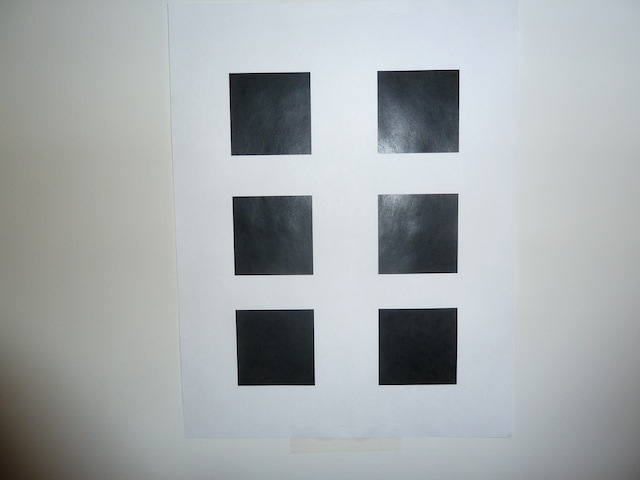
\includegraphics[width=0.45\linewidth]{figures/calib1.jpg}
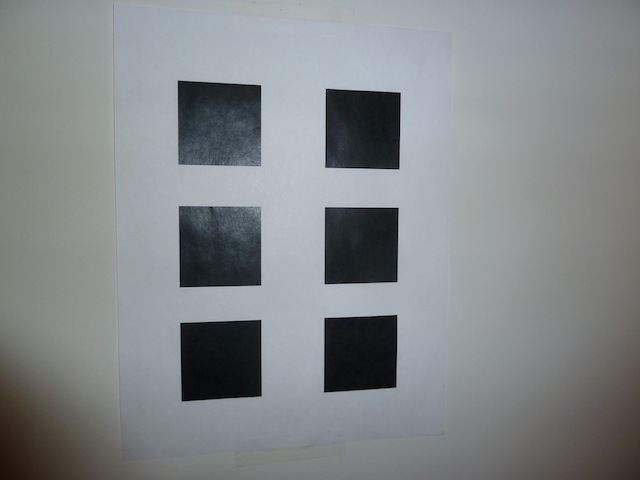
\includegraphics[width=0.45\linewidth]{figures/calib2.jpg}
\end{center}
\caption{Different calibration angles for Zhang's method}
\label{calib_pics}
\end{figure}

We used multiple views and took the average over different permutations. We found the following intrinsic parameter matrix $K$ for this camera:
\begin{equation*}
K =
  \left[ {\begin{array}{ccc}
   360.506 & -38.7974 & 128.692  \\
  0 & 470.953 & 162.864 \\
   0 & 0 & 1 \\
  \end{array} } \right]
\end{equation*}

\subsection{Reconstruction of Zhang's images}
We first reconstructed the images provided by Zhang~\cite{Calibration} because we were provided with the pictures and internal parameters. This provides us with proof that our algorithm works with another camera other than our own. Similarly, we wanted to have a baseline reconstruction to ensure that our camera calibration was mostly accurate. Figure~\ref{zhang_original} shows two original images from different views used for the reconstruction. Figure~\ref{zhang_nocorners} shows views of the 3D reconstructed object without including the corners as features. We can see that the normals of the different planes are pretty well represented as the normals appear to be almost perpendicular to each other. Similarly, the edge of the box is also pretty well reflected in our reconstruction. However, we did not include the corners, which were not detected by SIFT, as a feature, so the box does not have the full rectangular shape. Figure~\ref{zhang_reconstructed} shows an improvement in the shape of the box when we included the corners as a feature.

\begin{figure}[H]
\begin{center}
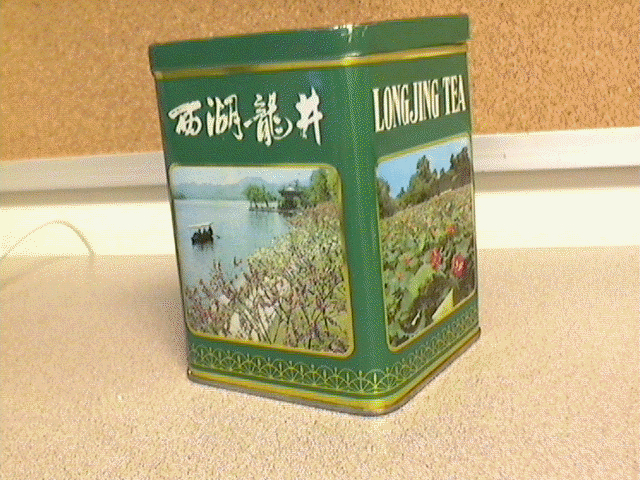
\includegraphics[width=0.45\linewidth]{figures/TeaBox1.jpg}
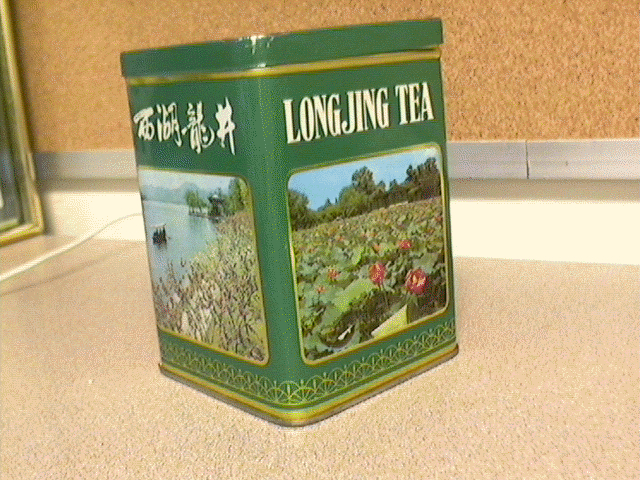
\includegraphics[width=0.45\linewidth]{figures/TeaBox2.jpg}
\end{center}
\caption{Original Zhang photos}
\label{zhang_original}
\end{figure}

\begin{figure}[H]
\begin{center}
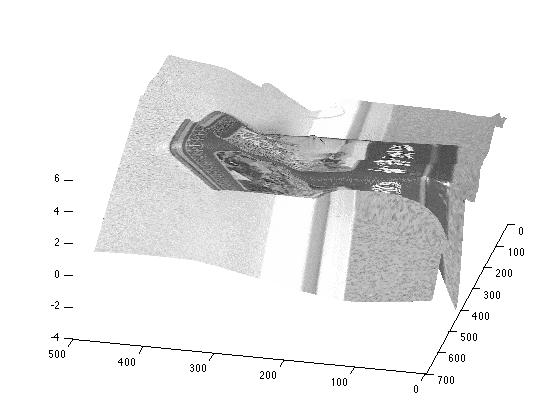
\includegraphics[width=0.45\linewidth]{figures/nocorners1.jpg}
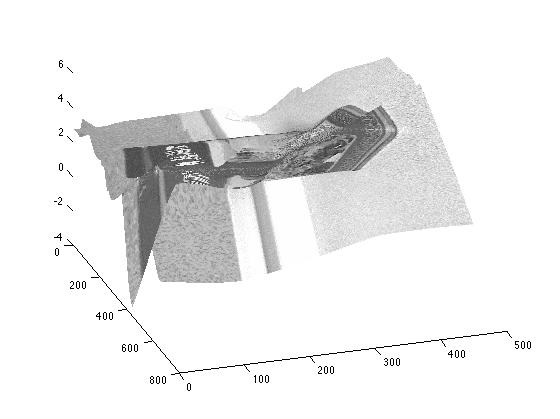
\includegraphics[width=0.45\linewidth]{figures/nocorners2.jpg}
\end{center}
\caption{3D reconstruction without corners included as features.}
\label{zhang_nocorners}
\end{figure}

\begin{figure}[H]
\begin{center}
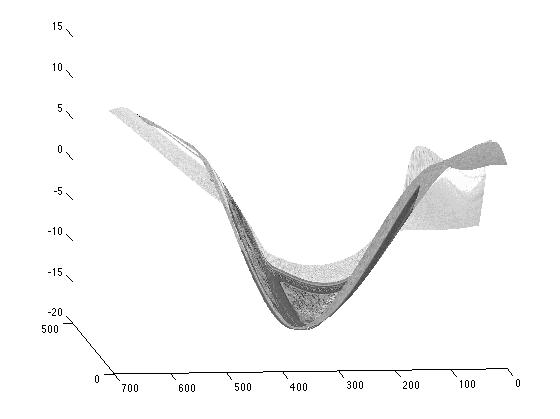
\includegraphics[width=0.45\linewidth]{figures/pic1.jpg}
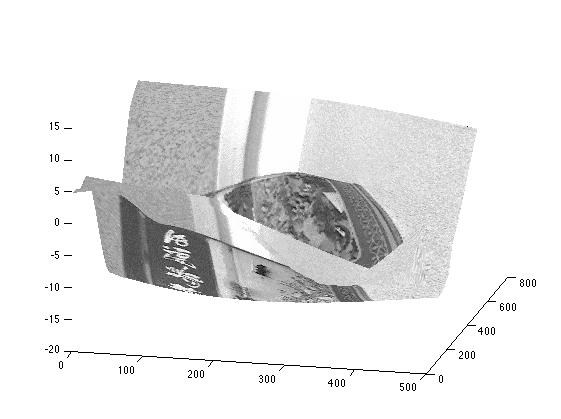
\includegraphics[width=0.45\linewidth]{figures/pic2.jpg}
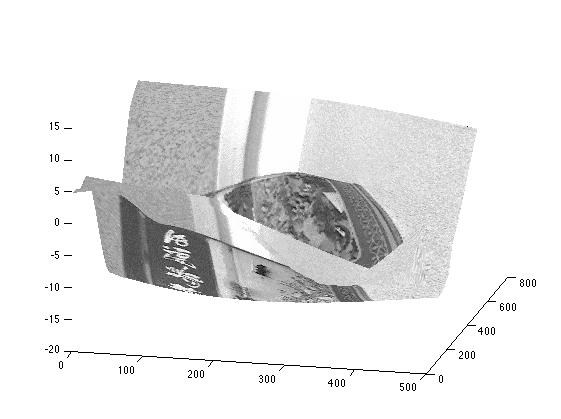
\includegraphics[width=0.45\linewidth]{figures/pic3.jpg}
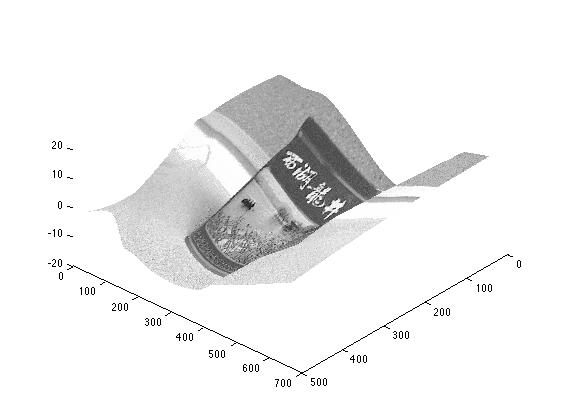
\includegraphics[width=0.45\linewidth]{figures/pic4.jpg}
\end{center}
\caption{Different views of 3D reconstructions with corners included as features.}
\label{zhang_reconstructed}
\end{figure}

\subsection{Our Reconstructions}
These are the reconstructions that we did with our own camera. Figure~\ref{original} has the original images, and Figure~\ref{sift_features} shows the matching points found by SIFT. Figure~\ref{kcup_nocorners} shows our reconstruction without including the corners as features. As we can see, like in the other reconstruction, the reconstruction is pretty representative of the object, but the shape is not very well preserved. However, with the addition of corners, the shape of the box becomes more representative of the actual object as seen in Figure~\ref{kcup_corners}. It is important to note that the reconstruction is not perfect because we only used two images, so we could only gather a limited number of information and constraints about the spatial points. This could be improved with more images and a more refined fundamental and essential matrix.

\begin{figure}[H]
\begin{center}
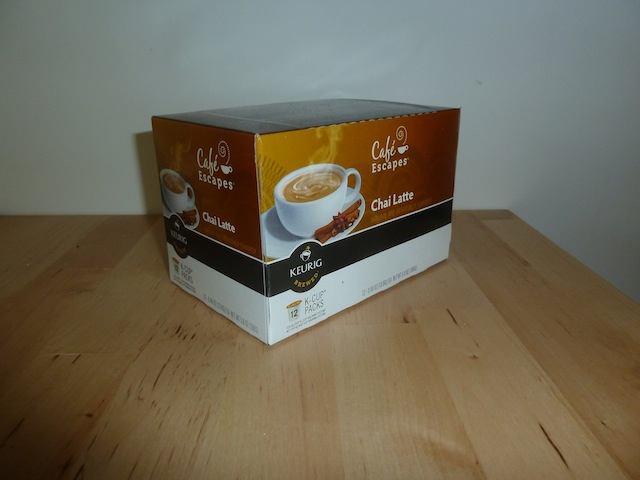
\includegraphics[width=0.45\linewidth]{figures/kcup1.jpg}
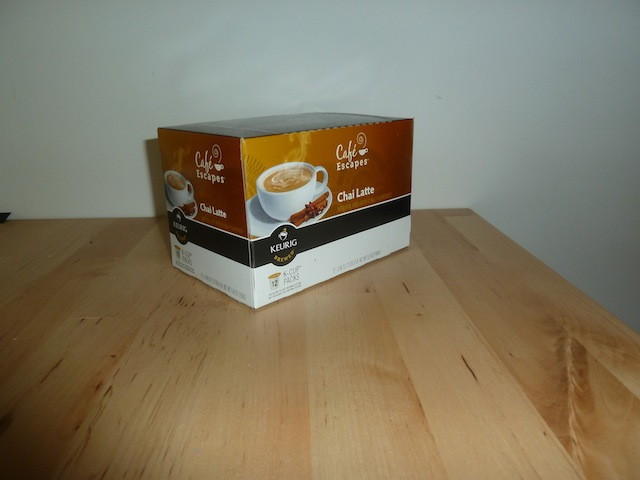
\includegraphics[width=0.45\linewidth]{figures/kcup2.jpg}
\end{center}
\caption{Original Images}
\label{original}
\end{figure}

\begin{figure}[H]
\begin{center}
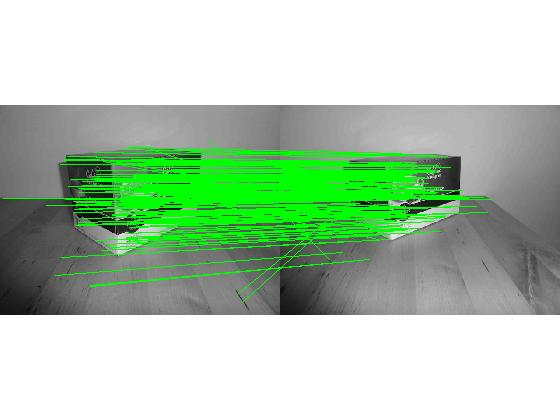
\includegraphics[width=0.95\linewidth]{figures/sift.jpg}
\end{center}
\caption{Matching points on images.}
\label{sift_features}
\end{figure}

\begin{figure}[H]
\begin{center}
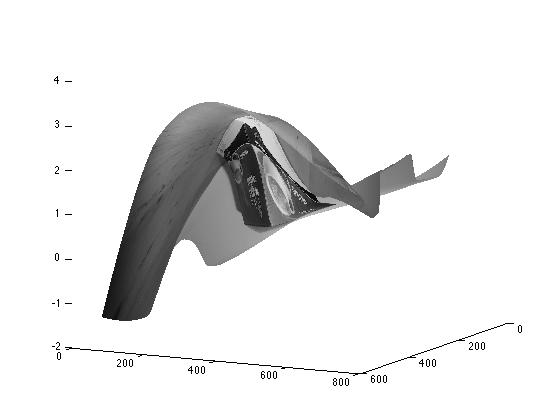
\includegraphics[width=0.45\linewidth]{figures/kcup_nocorners1.jpg}
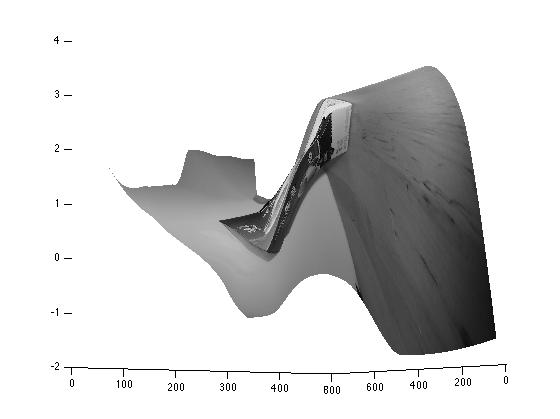
\includegraphics[width=0.45\linewidth]{figures/kcup_nocorners2.jpg}
\end{center}
\caption{3D reconstruction without corners as features.}
\label{kcup_nocorners}
\end{figure}

\begin{figure}[H]
\begin{center}
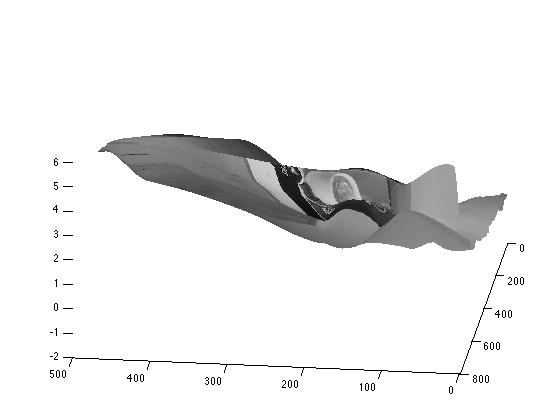
\includegraphics[width=0.45\linewidth]{figures/kcup_corners1.jpg}
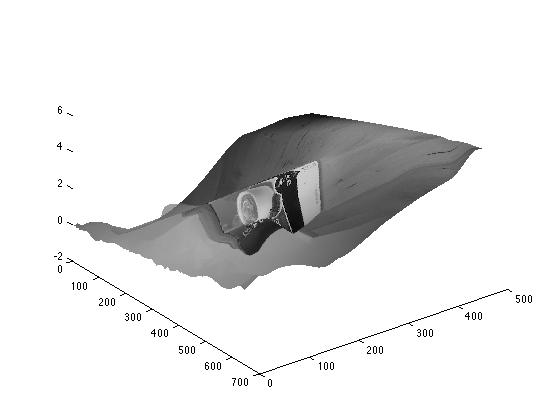
\includegraphics[width=0.45\linewidth]{figures/kcup_corners2.jpg}
\end{center}
\caption{3D reconstruction with corners as features.}
\label{kcup_corners}
\end{figure}
